\documentclass{beamer}
\usecolortheme{beaver}

\usepackage{amssymb}
\usepackage{pgfplots} 
\usepackage{graphicx}
\usepackage[utf8x]{inputenc}
\usepackage{tikz}
\usepackage{bbm}
\usepackage{subcaption}
\usepackage{mathtools}
\usepackage{lipsum}
\DeclarePairedDelimiter{\ceil}{\lceil}{\rceil}
\newcommand{\eqtext}[1]{\ensuremath{\stackrel{#1}{=}}}
\newcommand{\leqtext}[1]{\ensuremath{\stackrel{#1}{\leq}}}
\newcommand{\N}{\mathbb{N}}
\newcommand{\R}{\mathbb{R}}
\newcommand{\E}{\mathbb{E}}
\newcommand{\epl}{\varepsilon}
\newcommand{\defeq}{\coloneqq}
\renewcommand{\phi}{\varphi}

\title{Uncertain Darcy's problem \\ and the stochastic particle transport}
\subtitle{Semester Project - Master in CSE}
\author{Giacomo Garegnani \\ {Supervisors: Dr. Sebastian Krumscheid and Prof. Fabio Nobile}}
\institute{EPFL}
\date{16/06/2016}

\begin{document}

\frame{\titlepage}

\begin{frame}
\frametitle{Problem statement}
Underground flow $\rightarrow$ Uncertain Darcy's problem
\begin{equation*}
	\left \{
  	\begin{aligned}
		u &= -A \nabla p, && \text{in } D, \\
		\nabla\cdot u &= f, && \text{in } D, \\
		p &= p_0, && \text{on } \Gamma_{in},\\
		p &= 0, && \text{on } \Gamma_{out}, \\
		\nabla p \cdot n &= 0, && \text{on } \Gamma_N,
	\end{aligned} \right.
\end{equation*}
Stochastic particle transport $\rightarrow$ Ornstein–Uhlenbeck process
\begin{equation*}
	\left \{
	\begin{aligned}
		dX(t) &= u(X(t)) dt + \sigma dW(t), && 0 \leq t \leq T, \\
		X(0) &= X_0 \in D, \\
	\end{aligned} \right.
\end{equation*}
\end{frame}

\begin{frame}
\frametitle{Outline}
\begin{itemize}
	\item Expected exit time from a domain
	\item Theoretical investigation: perturbed SDE's 
	\item The uncertain Darcy's problem 
\end{itemize}
\end{frame}

\begin{frame}
\frametitle{Mean exit time. Setting}
Given a domain $D \subset \R^d$, $f\colon D \to \R^d, g\colon D \to \R^{d \times m}$ and an $m$-dimensional standard Wiener process $W(t)$, consider
\begin{equation*}
\left \{
\begin{aligned}
	dX(t) &= f(X(t)) dt + g(X(t))dW(t), && 0 < t \leq T, \\
	X(0)  &= X_0, && X_0 \in D.
\end{aligned} \right .
\end{equation*}
The equation is defined in a domain $D$ $\rightarrow$ boundary conditions
\begin{itemize}
	\item \textit{killing boundaries}: $X(t)$ is stopped,
	\item \textit{reflecting boundaries}: $X(t)$ is reflected normally inside $D$.
\end{itemize}
\end{frame}

\begin{frame}
\frametitle{Mean exit time. Problem statement}
\underline{Problem}. Estimate the exit time of the trajectories
\begin{equation*}
	\tau = \min\{\tau_e,T\}, \text{ where } \tau_e = \min\{t\colon X(t)\notin D\}.
\end{equation*}
Another quantity of interest, given $F\colon D \to \R$
\begin{equation*}
	\phi = \phi(T,X_0,F) = \mathbbm{1}_{\{T < \tau_e\}}F(X(T)).
\end{equation*}
If $F \equiv 1$, exit probability 
\begin{equation*}
	\Phi(T,X_0) \defeq \Pr(\tau < T | X(0) = X_0) = 1 - \mathbb{E}(\phi(T,X_0,1)). 
\end{equation*}
\underline{Goal}. Estimate numerically $\tau$ and $\phi$.
\end{frame}

\begin{frame}[plain]
\frametitle{Discrete Euler-Maruyama}
Method:
\begin{equation*}
	\left \{
	\begin{aligned}
		X_h^d(t_{i+1}) &= f(X(t_i))h + g(X(t_i))(W(t_{i+1}) - W(t_{i})),  \\
		X_h^d(0) &= X_0.
	\end{aligned} \right .
\end{equation*}
Parameters of interest computed naively
\begin{equation*}
\begin{aligned}
	\tau_h^d &= \min\{\tau_{h,e}^d,T\}, \text{ where } \tau_{h,e}^d = \min \{t_i \colon X_h^d(t_i) \notin D\}, \\
	\phi_h^d &= \mathbbm{1}_{\{T < \tau_{h,e}^d\}}F(X_h^d(T)).
\end{aligned}
\end{equation*}
Missed exits $\Rightarrow$ 1/2 loss in weak order:
\begin{align*}
	|\mathbb{E}(\tau_h^d) - \mathbb{E}(\tau)| &= O(\sqrt{h}), \\
	|\mathbb{E}(\phi_h^d) - \mathbb{E}(\phi)| &= O(\sqrt{h}).
\end{align*}	
\end{frame}

\begin{frame}[plain]
\frametitle{Continuous Euler-Maruyama}
\underline{Goal}. Restore the order of convergence 1 of Euler-Maruyama in $\R^d$ $\Rightarrow$ Brownian bridge approach.

Method:
\begin{equation*}
	\left \{
	\begin{aligned}
		X_h^c(t) &= f(X(t_i))(t-t_i) + g(X(t_i))(W(t) - W(t_{i})),  && t_i < t \leq t_{i+1},\\
		X_h^c(0) &= X_0.
	\end{aligned} \right .
\end{equation*} 
Estimate at each time step the probability of exit. If $D$ is an half-space
\begin{equation*}
\begin{aligned}
	&\Pr (\exists t \in [ t_i,t_{i+1} ] \quad X_h^d(t) \notin D | X_h^d(t_i) = x_i, X_h^d(t_{i+1}) = x_{i+1}) \\
	&\quad = p(x_i,x_{i+1},h) \\
	&\quad = \exp\Big(-2\frac{[n\cdot(x_i - z_i)][n\cdot(x_{i+1} - z_i)]}{hn\cdot (gg^T(x_i)n)}\Big),
\end{aligned}
\end{equation*}
\end{frame}

\begin{frame}
\frametitle{Continuous Euler-Maruyama}
Parameters of interest. Given $u$ a realization of $U$ uniform r.v. in $(0,1)$
\begin{equation*}
\begin{aligned}
	\tau_h^c &= \min \{T,\tau_{h,e}^c\}, \\
	\text{ where } \tau_{h,e}^c &= \min\{\tau_{h,e1}^c, \tau_{h,e2}^c\}, \\
	\tau_{h,e1}^c &= \min\{t_i = hi \colon X_h(t_i) \notin D\}, \\
	\tau_{h,e2}^c &= \min\{t_i = hi \colon u < p(x_{i-1},x_i,h) \}, \\
	\phi_h^c &= \mathbbm{1}_{\{T < \tau_{h,e}^c\}}F(X_h^c(T)).
\end{aligned}
\end{equation*}
Weak order 1 is restored:
\begin{align*}
	|\mathbb{E}(\tau_h^c) - \mathbb{E}(\tau)| &= O(h), \\
	|\mathbb{E}(\phi_h^c) - \mathbb{E}(\phi)| &= O(h).
\end{align*}
\end{frame}

\subsection{A PDE approach}\label{sec:PDEs}
It is possible to express the exit time and the probability of exit from a domain in terms of the solution of partial differential equations (PDE's).
Let us denote by $\Gamma_k,\Gamma_r$ the killing and reflecting subsets of $\partial D$. We consider then the expectation of the exit time from the domain $D$ for a trajectory that at $t=0$ is at position $x$, \textit{i.e.},
\begin{equation}\label{eq:ExpTau}
	\bar\tau = \mathbb{E}(\tau | X(0) = x).
\end{equation}
Let us define the operator $\mathcal L$ induced by \eqref{eq:GeneralModel} acts on a function $u\colon \mathbb{R}^d \rightarrow \mathbb{R}$  as follows
\begin{equation}\label{eq:LOperator}
	\mathcal Lu = f \cdot \nabla u + \frac{1}{2} gg^T : \nabla \nabla u,
\end{equation}
where the $:$ operator between two matrices $A,B$ in $\mathbb{R}^{d\times d}$ is defined as follows
\begin{equation}\label{eq:twoPoints}
	A : B = \sum_{i,j = 1}^d \{A\}_{ij}\{B\}_{ij} = \text{tr}(A^TB).
\end{equation}
It is possible to show \cite{Krumscheid2015,Pavliotis2014} that $\bar\tau$ is the solution of the following partial differential equation 

\begin{theorem} Let $\mathcal L$ be the differential operator defined as \eqref{eq:LOperator}. Then, the mean exit time $\bar \tau$ is the solution of the following boundary value problem
\begin{equation}\label{eq:PDETau}
\begin{cases}
	\mathcal L \bar \tau = -1, & \text{in } D, \\
	\bar\tau = 0 & \text{on } \Gamma_k, \\
	\nabla \bar\tau \cdot n = 0 & \text{on } \Gamma_r.
\end{cases}
\end{equation}
\end{theorem}
Further analytical treatement of the mean exit time can be found in \cite{Krumscheid2015,Pavliotis2014}. \\
We now consider the probability of exit from $D$ for a solution $X(t)$ that is equal to $x$ for $t = s < T$. This probability is the solution of a boundary value problem.
\begin{theorem} Let $\mathcal L$ be the differential operator defined as \eqref{eq:LOperator}. Then
\begin{equation}\label{eq:ExitProbNotation}
	\Pr(\tau < T | X(s) = x) = \Phi(x,s,T) 
\end{equation}
where $\Phi(x,s,T)$ is the solution of the following problem
\begin{equation}\label{eq:PDEPhi}
\begin{cases}
	\frac{\partial}{\partial t} \Phi(x,t,T) + \mathcal L \Phi(x,t,T) = 0 & \text{in } D, t < T, \\
	u(x,t,T) = 1 & \text{on } \partial D, \\
	u(x,T,T) = 0 & \text{in } D.
\end{cases}
\end{equation}
\end{theorem}
Further treatment and the proof of this result can be found in \cite{Sirovich2010}. It is therefore possible to approximate $\bar\tau$ and $\Phi$ by means of classical methods for solving PDE's numerically, such as finite differences or the Finite Elements Method.


\begin{frame}
\frametitle{One-dimensional case - Setup}
Consider $D=[-1,1]$ and the SDE
\begin{equation*}
\left \{
\begin{aligned}
	dX(t) &= f(X(t)) dt + g(X(t))dW(t), && 0 < t \leq T, \\
	X(0)  &= X_0, && X_0 \in D.
\end{aligned} \right .
\end{equation*}
Set mixed boundary conditions and
\begin{equation*}
\begin{split}
	f(x) &= -V'(x), \text{ where } V(x) = 0.1(8x^4 - 8x^2 + x + 2), \\
	g(x) &= \sigma \in \R.
\end{split}
\end{equation*}
\underline{Goal}. Verify the weak order of convergence of DEM and CEM.
\underline{Reference solution}. Solution of PDE's
\begin{itemize}
	\item Analytic solution in one-dimensional case for $\bar \tau$,
	\item Finite Differences for $\Phi$.
\end{itemize}
\end{frame}

\begin{frame}
\frametitle{One-dimensional case - Results}
\begin{figure}[t]
    \centering
    \begin{subfigure}{0.49\linewidth}
        \centering
        \resizebox{1\linewidth}{!}{\input{Pictures/OneDTau.tikz} }  
        \caption{Approximation of $\tau$}
        \label{fig:KillOneDPhi}
    \end{subfigure}
    \begin{subfigure}{0.49\linewidth}
        \centering
        \resizebox{1\linewidth}{!}{\input{Pictures/OneDPhi.tikz} }  
        \caption{Approximation of $\Phi$}
        \label{fig:ReflectOneDPhi}
    \end{subfigure}    
    \caption{Results for the one-dimensional case.}
\end{figure}
\end{frame}

\begin{frame}
\frametitle{One-dimensional case - Results}
\begin{figure}[t]
    \centering
    \begin{subfigure}{0.49\linewidth}
        \centering
        \resizebox{1\linewidth}{!}{\input{Pictures/OneDTauProf.tikz} }  
        \caption{Approximation of $\tau$}
        \label{fig:KillOneDPhi}
    \end{subfigure}
    \begin{subfigure}{0.49\linewidth}
        \centering
        \resizebox{1\linewidth}{!}{\input{Pictures/OneDPhiProf.tikz} }  
        \caption{Approximation of $\Phi$}
        \label{fig:ReflectOneDPhi}
    \end{subfigure}    
    \caption{Approximation of $\tau$ and $\Phi$ with respect to initial value $X_0$.}
\end{figure}
\end{frame}

\begin{frame}
\frametitle{Two-dimensional case - Setup}
Consider $D=[-1,1]^2$ and the SDE
\begin{equation*}
\left \{
\begin{aligned}
	dX(t) &= f(X(t)) dt + g(X(t))dW(t), && 0 < t \leq T, \\
	X(0)  &= X_0, && X_0 \in D.
\end{aligned} \right .
\end{equation*}
Setting:
\begin{itemize}
	\item Mixed boundary conditions, \\
	\item $f = 0$ $\to$ pure Brownian motion.
\end{itemize}
\underline{Goal}. Verify the weak order of convergence of DEM and CEM. \\
\underline{Reference solution}. Solution of PDE's with FEM.
\end{frame}

\begin{frame}
\frametitle{Two-dimensional case - Results}
\begin{figure}[t]
    \centering
    \begin{subfigure}{0.49\linewidth}
        \centering
        \resizebox{1\linewidth}{!}{\input{Pictures/TwoDTau.tikz} }  
        \caption{Approximation of $\tau$}
        \label{fig:KillOneDPhi}
    \end{subfigure}
    \begin{subfigure}{0.49\linewidth}
        \centering
        \resizebox{1\linewidth}{!}{% This file was created by matlab2tikz.
%
%The latest updates can be retrieved from
%  http://www.mathworks.com/matlabcentral/fileexchange/22022-matlab2tikz-matlab2tikz
%where you can also make suggestions and rate matlab2tikz.
%
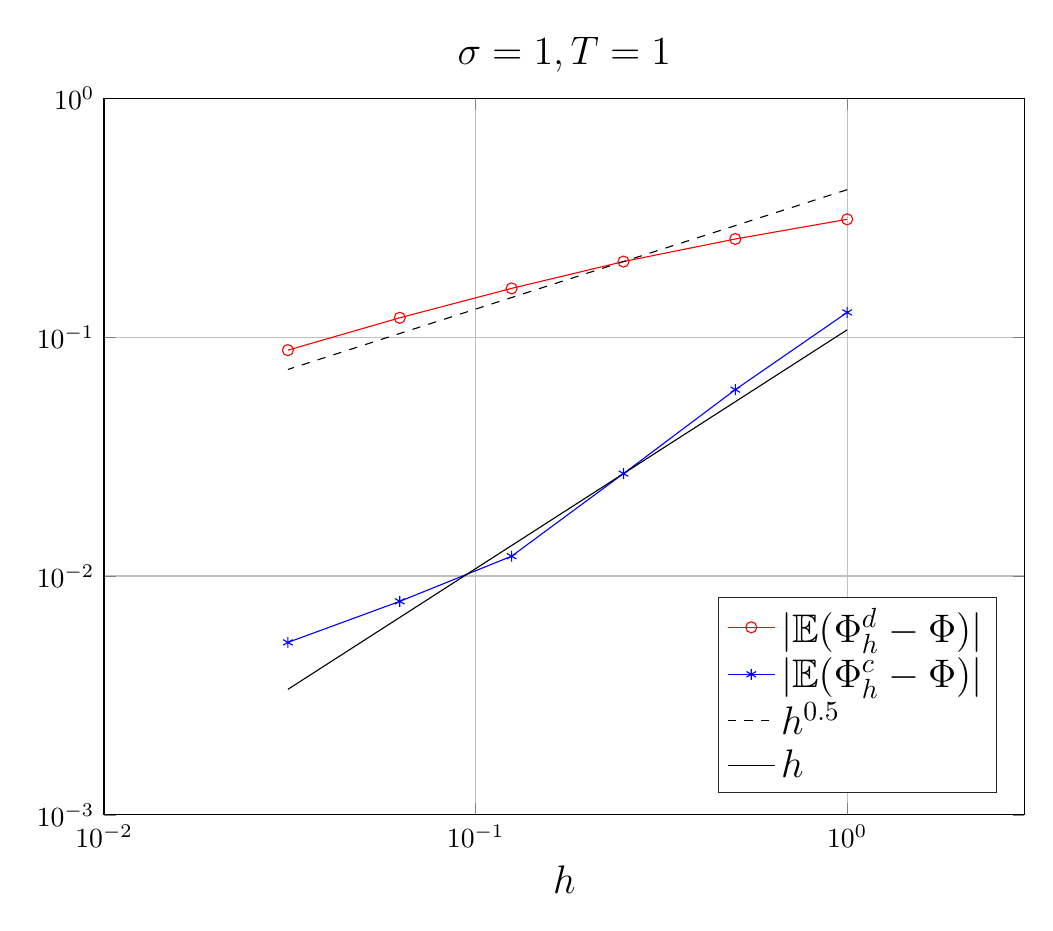
\begin{tikzpicture}

\begin{axis}[%
width=4.602in,
height=3.583in,
at={(0.772in,0.484in)},
scale only axis,
title={$\sigma = 1, T = 1$},
title style = {font=\Large},
xmode=log,
xmin=0.01,
xmax=3,
xminorticks=false,
xlabel={$h$},
xlabel style={font=\Large},
xmajorgrids,
ymode=log,
ymin=0.001,
ymax=1,
yminorticks=false,
ymajorgrids,
axis background/.style={fill=white},
legend pos = south east,
legend style={legend cell align=left,align=left,draw=white!15!black,font=\Large}
]
\addplot [color=red,solid,mark=o,mark options={solid}]
  table[row sep=crcr]{%
1	0.31134162505938\\
0.5	0.25753162505938\\
0.25	0.20716162505938\\
0.125	0.15999162505938\\
0.0625	0.12047162505938\\
0.03125	0.0881916250593803\\
};
\addlegendentry{$|\E(\Phi_h^d - \Phi)|$};

\addplot [color=blue,solid,mark=asterisk,mark options={solid}]
  table[row sep=crcr]{%
1	0.12689162505938\\
0.5	0.0602816250593803\\
0.25	0.0268316250593803\\
0.125	0.0121016250593803\\
0.0625	0.00783162505938029\\
0.03125	0.00527162505938028\\
};
\addlegendentry{$|\E(\Phi_h^c - \Phi)|$};

\addplot [color=black,dashed]
  table[row sep=crcr]{%
1	0.41432325011876\\
0.5	0.292970779762226\\
0.25	0.20716162505938\\
0.125	0.146485389881113\\
0.0625	0.10358081252969\\
0.03125	0.0732426949405564\\
};
\addlegendentry{$h^{0.5}$};

\addplot [color=black,solid]
  table[row sep=crcr]{%
1	0.107326500237521\\
0.5	0.0536632501187606\\
0.25	0.0268316250593803\\
0.125	0.0134158125296902\\
0.0625	0.00670790626484508\\
0.03125	0.00335395313242254\\
};
\addlegendentry{$h$};

\end{axis}
\end{tikzpicture}%
 }  
        \caption{Approximation of $\Phi$}
        \label{fig:ReflectOneDPhi}
    \end{subfigure}    
    \caption{Results for the two-dimensional case.}
\end{figure}
\end{frame}



	
\end{document}
